\section{February 9, 2021}

\subsection{Recap of hyperbolic space}
Last time we talked about how to view a hyperbolic space a couple different ways, listed below. (For now we limit our attention to $\H^2$, but in $n$ dimensions arguments work pretty much the same way.)
\begin{enumerate}[label=(\arabic*)]
    \item The hyperboloid model. Here we consider the upper half plane $z^2=x^2+y^2+1$ (for $z\geq 1$) sitting in $\R^3$, with the metric $ds^2=dx^2+dy^2-dz^2$.
    \item The Klein-Beltrami model. Consider the disk $u^2+v^2<1$, with the metric $d^2=$ something messy. 
    \item The Poincare disk model. Once again consider $u^2+v^2<1$, with the metric $ds ^2 = \frac{4(du^2+dv^2)}{(1-u^2-v^2)^2}$.
    \item The upper half plane. Consider all pairs $(x,y)$ for $y>0$, with the metric $d^2 = \frac{dx^2+dy^2}{y^2}$.
\end{enumerate}
\begin{figure}[H]
\centering
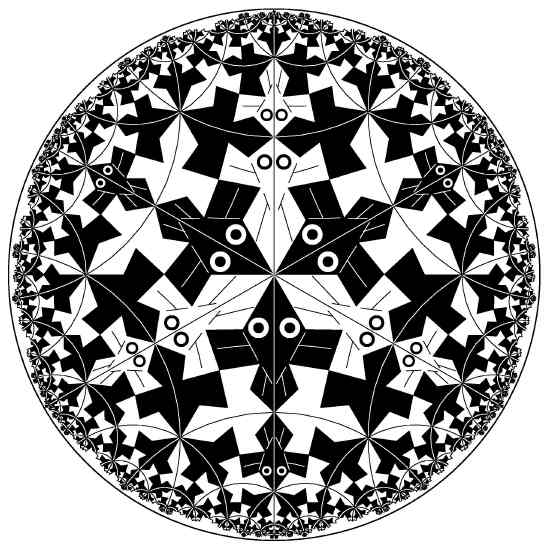
\includegraphics[width=0.5\linewidth]{figures/escher.jpg}
\label{escher} 
\caption{Obligatory Escher print.} 
\end{figure}
This tells us a couple of things: all the little dudes are the same size. You can also track straight lines on the disk, the diameter lines definitely are but so are the arcs outlined in \cref{escher}. It looks a little funny because this is a disk of infinite volume; the metric gets closer to zero as you approach the boundary, and if you try to integrate from the center out you'll see that it diverges.

\subsection{The upper half plane}
Let $x,y$ for $y>0$. It's easier to package them in a complex number $z=x+iy$. So our metric is given by \[
    ds^2 = \frac{dx^2+dy^2}{y^2}= \frac{dz\, d\overline{z}}{(\operatorname{Im}z)^2}=\frac{|dz|^2}{(\operatorname{Im}z)^2}.
\] We claim there is a natural group acting on this space, namely $\operatorname{SL}(2,\R):= \left\{\left( 
\begin{smallmatrix}
    a & b \\ c & d
\end{smallmatrix}\right) \,\big | \,ad-bc=1 \right\} $. This acts on $\C$ by the rule $\left( 
\begin{smallmatrix}
    a & b \\ c & d
\end{smallmatrix}\right) \cdot z= \frac{az+b}{cz+d}$. You can think of this action as $
\left( 
\begin{smallmatrix}
    a & b \\ c & d
\end{smallmatrix}\right) \left( 
\begin{smallmatrix}
    z \\ 1
\end{smallmatrix}\right) =\left( 
\begin{smallmatrix}
    az+b \\ cz+d
\end{smallmatrix}\right) $, so when the matrix acts on $z$ itself, it transforms the ratio of $z:1$ to $az+b: cz+d$. If you think about the linear action of matrices on $\C^2$ and the induced action it has on quotients, this is really an action on $\C\mathrm P^1$. Call this ratio $\frac{az+b}{cz+d}=w$, and this transformation is called a \textbf{M\"obius transformation}. Does this really take the upper half plane to the upper half plane? To do this, let's see if $\operatorname{Im}w=(w-\overline{w})$\footnote{It's actually $\frac{w-\overline{w}}{2i}$, but we're just trying to check whether it's positive or not.} is positive. We have 
\begin{align*}
    w-\overline{w}&=\frac{az+b}{cz+d}-\frac{a\overline{z}+b}{c\overline{z}+d}\\
                  &= \frac{z-\overline{z}}{|cz+d|^2}.
\end{align*}\footnote{Some algebra was skipped.}So $\operatorname{Im}w= \frac{\operatorname{Im}z}{|cz+d|^2}>0$, and this action is really a transformation of the upper half plane. Further more, this is a local isometry. Since $w=\frac{az+b}{cz+d}$, $dw=\frac{a(cz+d)-c(az+b)}{(cz+d)^2}dz=\frac{dz}{(cz+d)^2}$. Similarly, $d\overline{w}= \frac{d\overline{z}}{(c\overline{z}+d)^2}$, and $dw \, d\overline{w}=\frac{dz \, d\overline{z}}{|cz+d|^4}$. But the imaginary part transforms by $\frac{1}{|cz+d|^2}$, so \[
\frac{|dw|^2}{(\operatorname{Im}w)^2}= \frac{|dz|^2}{(\operatorname{Im}z)^2},
\] and our metric is preserved. We have just shown that we have a group acting on the upper half plane by isometries; the next question to ask is ``is the action transitive?'' Here are some particularly interesting elements of $\operatorname{SL}(2,\R)$. 
\begin{itemize}
    \item $
        \begin{pmatrix}
            1 & a \\ 0 & 1
        \end{pmatrix}$: this sends $z \mapsto  z+a$, which translates $z$ by $a$ in the \emph{real} direction.
    \item $
        \begin{pmatrix}
            \sqrt{b} & 0 \\ 0 & \frac{1}{\sqrt{b}  } 
        \end{pmatrix}$: this sends $z \mapsto bz$, which scales $z$ by $b$.
\end{itemize}
If you consider $i$ as a ``center'' point for your model, we have $
\left( 
\begin{smallmatrix}
    1 & a \\ 0 & 1
\end{smallmatrix}\right) \left( 
\begin{smallmatrix}
    \sqrt{b} & 0 \\ 0 & 1 /\sqrt{b} 
\end{smallmatrix}\right) \cdot i=a+bi$, and composing the matrices gives $\left( 
\begin{smallmatrix}
    \sqrt{b} & a / \sqrt{b} \\ 0 & 1 / \sqrt{b} 
\end{smallmatrix}\right) $ as the map sending $i \mapsto a+bi$. Our action is transitive, since $i$ goes to any point, and the inverse matrix sends any point to $i$. Then any point gets sent to any point by first sending it to $i$, then the other point.

The next question to ask is ``what is the isotropy group of a point?'' We have \[
\begin{pmatrix}
    a & b \\ c & d
\end{pmatrix}i=i,\quad \frac{ai+b}{ci+d}=i\ \implies \ ai+b=di-c.
\] Then $a=d$ and $c=-b,$ so we are looking at matrices of the form $\left( 
\begin{smallmatrix}
    a & b \\ -b & a
\end{smallmatrix}\right) $; furthermore these matrices have determinant 1, so $a^2+b^2=1$. This becomes all matrices of the form $\left( 
\begin{smallmatrix}
    \cos \theta & \sin \theta \\ -\sin \theta & \cos \theta
\end{smallmatrix}\right) $, which is just $\operatorname{SO}(2)$. The point is applying one of these matrices to $i$ rotates the plane by $2 \theta$. Note that \[
i \mapsto \frac{\cos \theta i + \sin \theta}{-\sin \theta i + \cos \theta}=\frac{ie^{-i \theta}}{e^{-i \theta}}.
\] The derivative map, how much you rotate tangent vectors, is $\frac{1}{(cz+d)^2}=\frac{1}{e^{-2i \theta}}=e^{2i \theta}$. In particular, if $\theta=\pi$, then we rotate back to $2\pi$. This is not intrinsic to $i$, in general, $\left( 
\begin{smallmatrix}
    -1 & 0 \\ 0 & -1
\end{smallmatrix}\right) z=z$. So $\operatorname{Isom}(\H^2)=\operatorname{SL}(2,\R) / \pm I=\operatorname{PSL}(2,\R)$, and
\begin{align*}
    \H &= \operatorname{SL}(2,\R) / \operatorname{SO}(2) \\
       &=\operatorname{PSL}(2,\R) / \operatorname{PSO}(2).
\end{align*}

\subsection{Geodesics}
Let $(M,g)$ be a Riemannian manifold, and $p, q \in M$. We want to define the distance from $p$ to $q$. The first thing we do is define distance along a path: think of a path $\gamma (t)$ such that $\gamma (t_0)=p$ and $\gamma (t_f)=q$. Then we define the \textbf{length} of $\gamma $ by \[
    L(\gamma )=\int_{t_0}^{t_f} \sqrt{g(\dot \gamma ,\dot \gamma )}  \, dt.
\] This doesn't depend on parametrization, if you reparametrize you get the same integral. Define the \textbf{distance} from $p$ to $q$ as 
\[
d(p,q)=\underset{\gamma }{\inf} \,L(\gamma ),
\] 
where $\gamma $ is a path from $p$ to $q$. Unfortunately, a \textbf{geodesic} has two meanings, and we use both. One is that a geodesic is a locally length minizing path. The second definition of the geodesic is something that minimizes a different functional called the \textbf{energy} of the path. Things that minimize energy are length minimizing paths parametrized at constant speed. So for every geodesic, there's a \emph{best} parametriation where you move along at constant speed, and we say ``geodesic'' we speak of that parametrization. For now we're just talking about geometric paths, and want something that minimizes length.

The geodesic joining two points is not always unique. Consider $\R^2 \setminus \{0\} $, and the line connecting $(-1,0)$ and $(1,0)$. There is no path of length 2 connecting them, since it would have to go through the origin (not in the space). You can find a path that takes a small detour, as small as you want, so the $\operatorname{inf}(\text{all paths} )$ still equals 2. But there is no geodesic from $(-1,0)$ to $(1,0)$. So geodesics don't always exist globally\footnote{They always exist for \emph{compact} manifolds.}: they do always exist locally however, which we will soon see.

\subsection{Geodesics in nice spaces}
Our three nice spaces are the plane, the sphere, and hyperbolic space.
\begin{enumerate}[label=(\arabic*)]
    \item Consider $p,q \in \R^2$ with $\gamma (0)=p$ and $\gamma (1)=q$. Can you show the shortest path is a straight line? (This was homework for diff geo.) Assume $p=(0,0)$ and $q=(1,0)$ for simplicity (since length is invariant under isometries, and the argument works for arbitrary lengths). If our path is given by $y=\gamma (x)$, then 
        \begin{align*}
            L(\gamma )&=\int_{0}^{1} \sqrt{1+\left( \frac{dy}{dx} \right)^2 }  \, dx\\
                      &\geq \int_{1}^{0} \sqrt{1}  \, dx=1.
        \end{align*}We get equality iff $y$ is constant, since wiggling in the $y$ direction only makes the $(dy /dx )^2$ factor bigger, increasing the length. (Wow this was a lot simpler than the diff geo proof.)
    \item Now we move to $S^2$. If $(\varphi ,\theta)$ parametrize the sphere, then $ds ^2= d \varphi ^2+ \sin ^2 \varphi (d \theta)^2$. (Figure out which coordinate corresponds to the azimuthal or whatever angle from that expression.) What's the shortest path from the north pole to a point $(\varphi ,\theta)$? We have 
        \begin{align*}
            &\int \sqrt{\left( \frac{d\varphi }{dt} \right) ^2+ \sin ^2 \varphi \left( \frac{d \theta}{dt} \right) ^2}  \, dt\\
            &\geq \int \left| \frac{d\varphi }{dt} \right|  \, dt\geq \varphi _{\text{final} }.
        \end{align*}This is the same argument as before: any wiggles in the $\theta$ direction only contribute to $(d \theta / dt)^2$, increasing the length. You also always want $d \varphi /dt=| d\varphi /dt|$, i.e. no doubling back. So the length minimizing path is when $\theta$ is constant and $\varphi $ is monotonic, i.e. you're going straight down the longitudinal line. This continues all the way down to the south pole. So we have just shown that a great circle is a geodesic. To parametrize this, you can send $t=\cos \theta(0,0,1)+\sin \theta\vec v$, where $\vec v$ lives on a great circle. 

        Suppose we start at some other point $p$ with tangent vector $v$, where $p \in \R^3$ and $p\perp v \in \R^3$. Can you find a geodesic that goes through $p$ along $v$? Geodesics are invariant under isometry, so send $p$ to the north pole. Now find a geodesic/great circle going through $v$, and rotate back. We have shown that $\gamma (t)= \cos (t)p+\sin (t)v$ is a geodesic. 

        Spherical triangles have area of the sum of the angles minus $\pi$. In a plane this sum minus $\pi$ is zero, but in the sphere it's not. (A neat proof is in the diff geo textbook/my diff geo notes.) 
        \begin{namedthing}{(Digression!)} 
            We never discussed what area means for a Riemannian manifold. The idea of area is that you chop things up into little pieces, and find the area of each piece. This is a parallelogram spanned by two vectors $v,w$. This is going to be some sort of determinant. We want
            \begin{align*}
                |v| |w|\sin \theta&=\sqrt{|v|^2|w|^2-|v|^2|w|^2\cos ^2\theta} \\
                                  &=\sqrt{(v\cdot v)(w\cdot w)-(v\cdot w)^2} \\
                                  &=\sqrt{g_{11}g_{22}-g_{12}^2} \\
                                  &=\sqrt{\det g} .
            \end{align*}We gave an argument for two dimensions, but the same thing works for arbitary dimensions. In general\[
            \int \sqrt{\det g}  \, d^n x= \operatorname{volume}.
            \] In the case of $S^2$, $g_{11}=1,g_{12}=g_{21}=0,g_{22}\sin ^2\varphi $. So $dA=\sin \varphi  d \varphi  d \theta$, and then simply integrate. For stereographic coordinates, $g_{11}=g_{22}=\frac{4}{(1+u^2+v^2)^2}, g_{12}=0$, so $\sqrt{\det} =\frac{4}{(1+u^2+v^2)}$. So $dA= (4 \,du\, dv) / (1+u^2+v^2)^2$. In the Poincare disk, just replace $u^2,v^2$ with minus signs. In the upper half plane, $g_{11}=g_{22}=\frac{1}{y^2}, g_{12}=0$, $\det =\frac{1}{y^r},\sqrt{\det} =\frac{1}{y^2},\ dA=\frac{1}{y^2}dx\,dy$.
        \end{namedthing}
    \item Now we turn our attention to hyperbolic space. Suppose we have two point $i, iy_1$. Then the geodesic is also a straight line, since 
        \[
        d= \int \frac{\sqrt{dx^2+dy^2} }{y}\geq \int_{1}^{y_1} \left| \frac{dy}{y}  \right| =\left| \ln |y_1|
    \right|        . \] This diverges as you approach the outer edge, and also as you approach the center. Now for arbitrary $p,q$, send $p \to i$ and rotate until $q$ winds up above $i$ by our aforementioned transformations. What happens when you send a line through an isometry? The translation $\left( 
    \begin{smallmatrix}
        1 & a \\ 0 &1
\end{smallmatrix}\right) $ shifts a vertical line to the right by a factor of $a$, while dilation $\left( 
\begin{smallmatrix}
    \sqrt{b} & 0 \\ 0 & 1/(\sqrt{b} )
\end{smallmatrix}\right) $ does nothing to a vertical line. Now for the Mobius transformation $\left( 
\begin{smallmatrix}
    a & b \\ c & d
\end{smallmatrix}\right) $, $z \mapsto \frac{az+b}{cz+d}$, as $z$ gets large, this is approximately $a /c$. As $z$ gets small, this is approximately $b / d$. So the image of a vertical line is going to be something that starts on the real axis at $b /d$ and goes to $a /d$ (you know $b /d$ and $a /c$ are distinct since $ad-bc=1$). The remarkable thing is that this turns out to be a circle centered at the midpoint $\left( b /d + a/ c\right) /2$, with radius $\left( a /c - b/ d\right) /2 = (ad-bc)/2cd= 1 /2cd$. So our geodesics are either vertical lines or semicircles.

\end{enumerate}

Consider an \textbf{ideal triangle}, which is the limit of a triangle as one of the vertices goes off to infinity.

\begin{figure}[H]
\centering
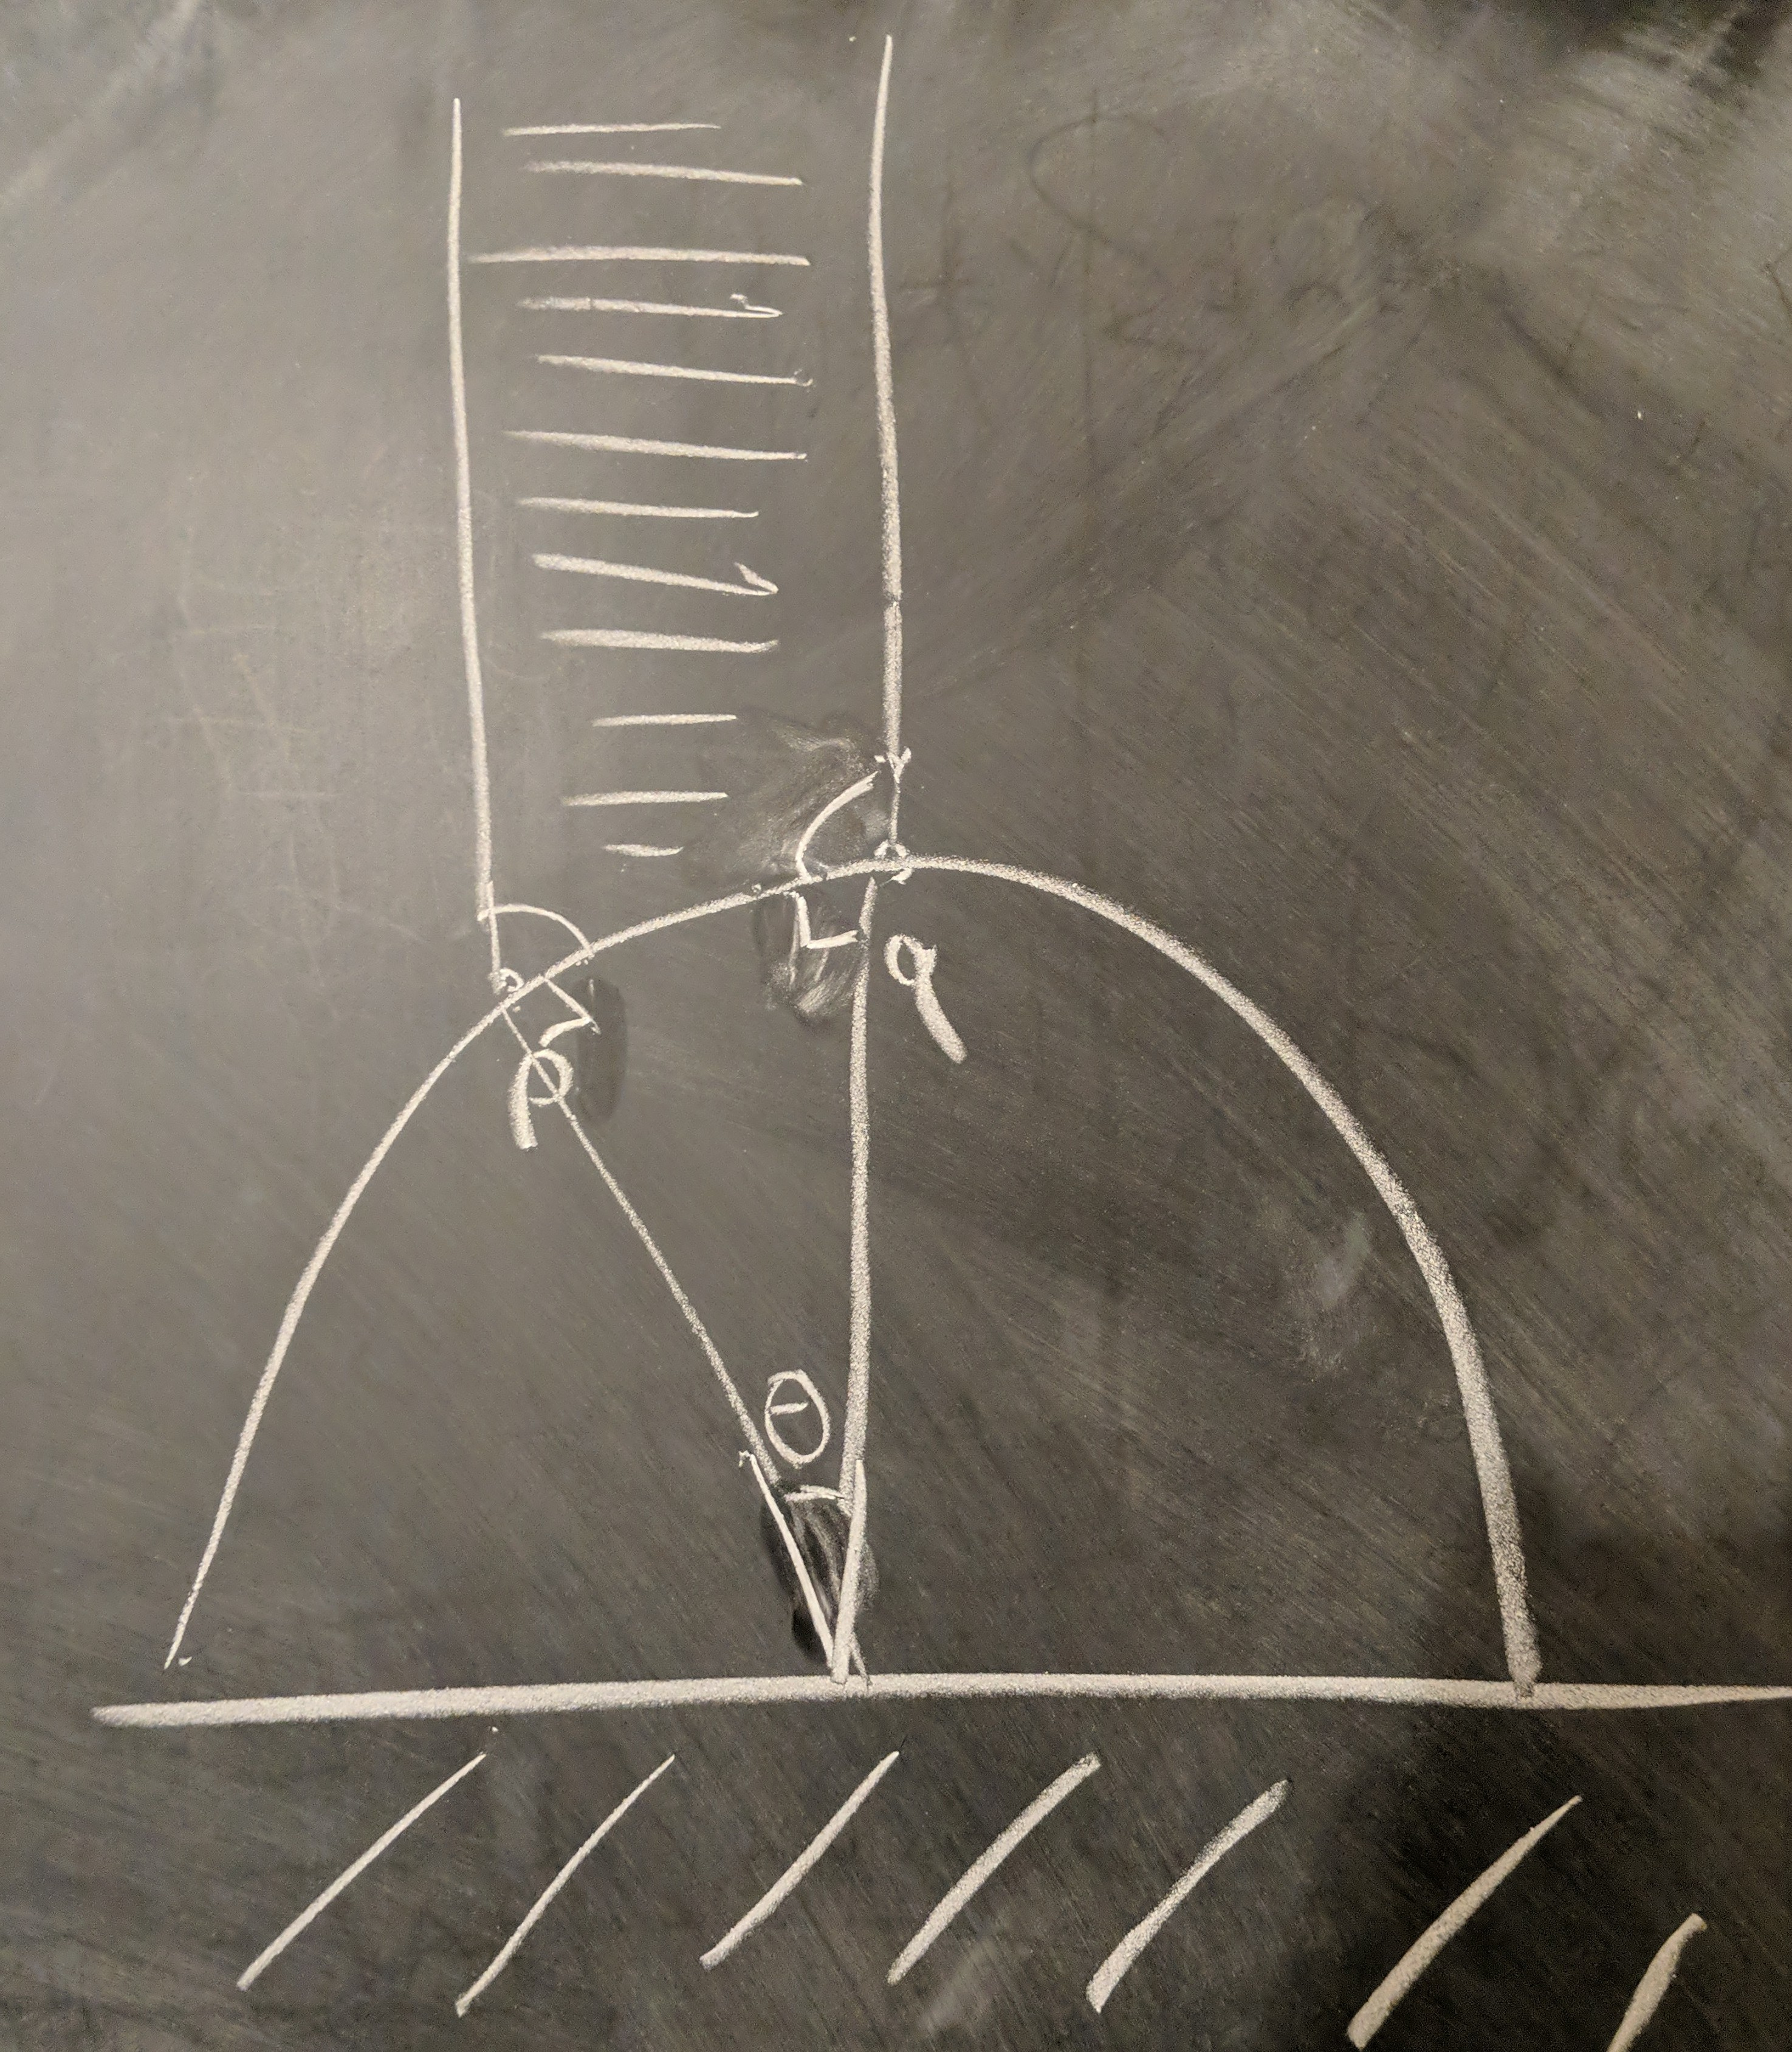
\includegraphics[width=0.4\linewidth]{figures/rgeo_lec7.1.jpg}
\end{figure}

The sum of the angles at $p$ and $q$ will be less than $\pi$. How much less? The claim is that it will be less than $\pi$ by exactly $\theta$, since summing up $\angle p,\angle q$, the right angles, and $\theta$ gives exactly $2 \pi$. The right angles plus $\theta$ is $\pi+\theta$, so $\angle p+\angle q=\pi -\theta$. 

How does this relate to areas? Recall that we want to integrate $\int \frac{dx\,dy}{y^2} =\int \frac{dx}{y}$, since $\int_{y_0}^{\infty} \frac{dy}{y^2}=\frac{1}{y_0}$. On a circle centered at the $x$-axis, $\int \frac{dx}{y}=\int  \, d\theta=\theta$. So in hyperbolic space, the angle deficit is the area. One last thing: usually you don't care about ideal triangles, you care about real triangles. Send it through an isometry takes one vertex to $i$, the other above $i$, and the third somewhere else.

\begin{figure}[H]
\centering
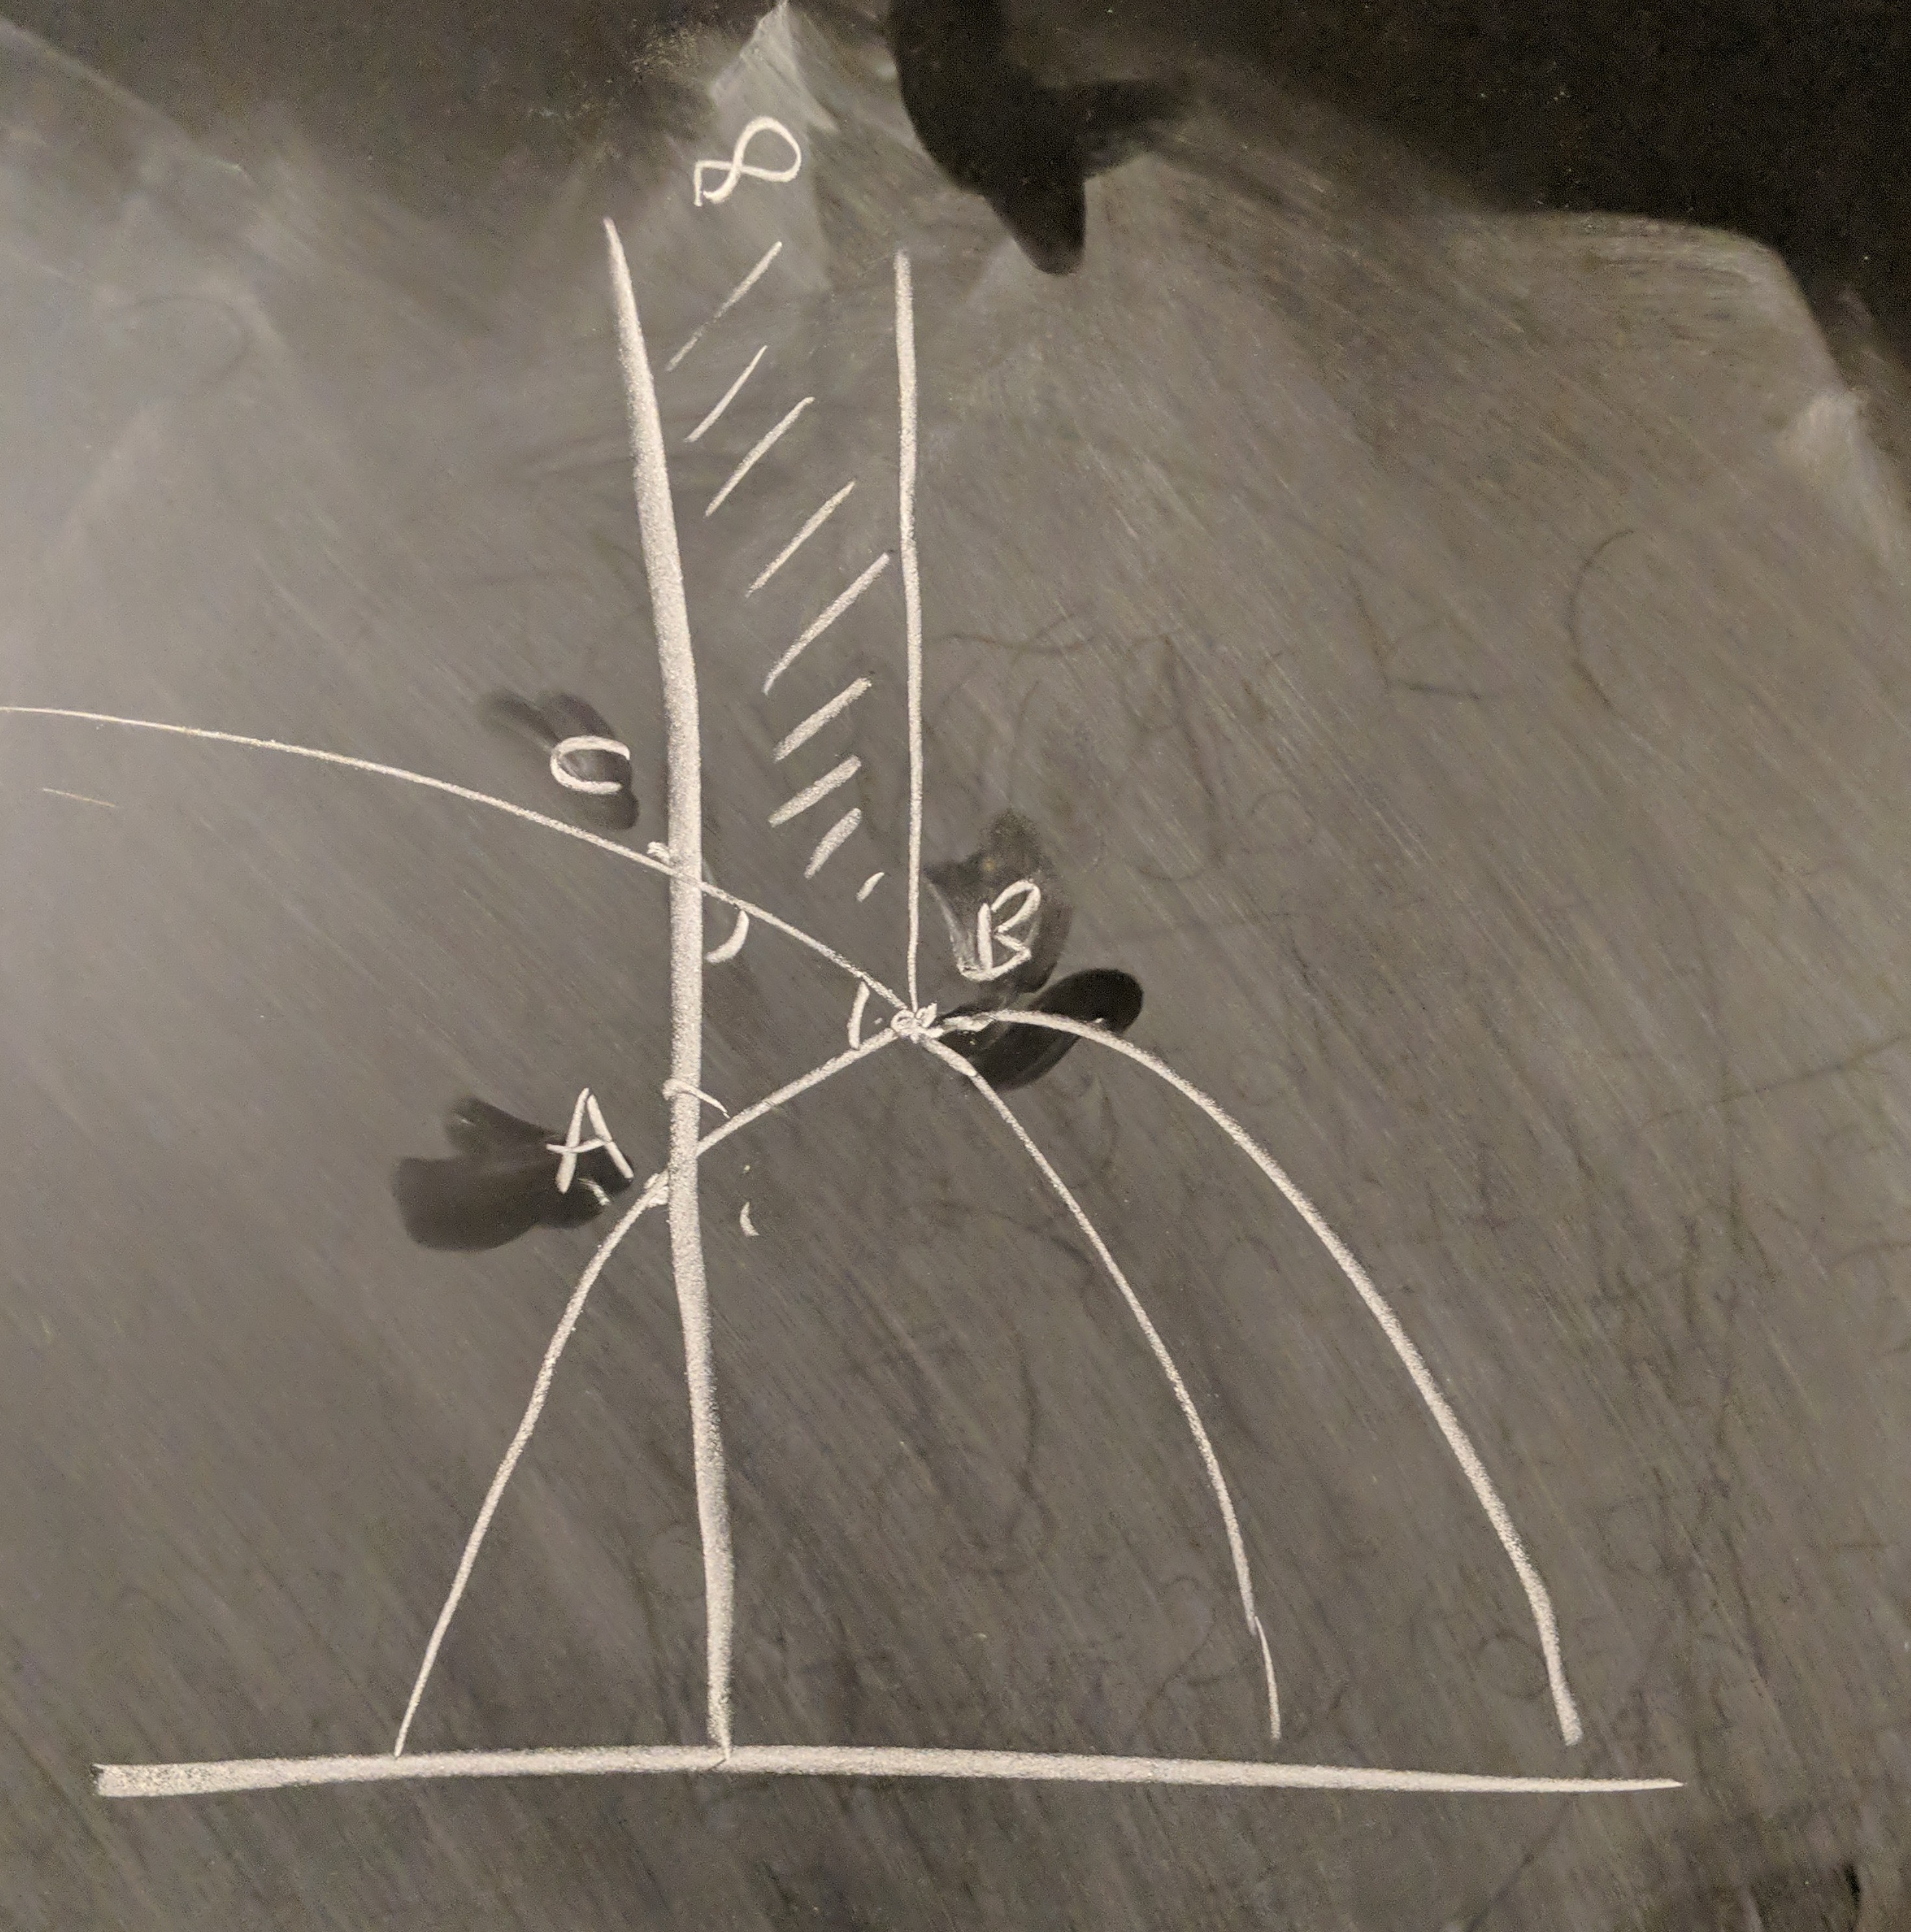
\includegraphics[width=0.4\linewidth]{figures/rgeo_lec7.2.jpg}
\end{figure}

The claim is that the sum of the angles of $\Delta ABC$ is the sum of the angles of $\Delta AB\infty$ (ideal triangle) \emph{minus} the sum of the angles of $\Delta BC \infty$  plus $\pi$. So the deficit for the real triangle is the deficit of the big ideal triangle minus the deficit of the little ideal triangle. Skipping some steps, we have shown that the sum of the angles in hyperbolic space is $\pi- \text{Area} \ \Delta$.

\begin{cor}
    The area of a triangle is less than $\pi$.
\end{cor}
Hyperbolic geometry is wack. See you next time.
